%%% Preamble starts here.
\documentclass{amsart}
%for the heading
\usepackage{fancyhdr, enumerate}
%for the picture. 
\usepackage{tikz, calc}
%adjust the page width
\usepackage[margin=1in]{geometry}

%% The next line says how the "vertex" style of nodes should look: drawn as small circles.
\tikzstyle{vertex}=[circle, draw, inner sep=0pt, minimum size=6pt]
%%
%% Next, we make a \vertex command as a shorthand in place of \node[vertex} to get that style.
\newcommand{\vertex}{\node[vertex]}

\linespread{1.1}

%command for double parentheses
\newcommand{\textmultiset}[2]{\bigl(\!{\binom{#1}{#2}}\!\bigr)}
\newcommand{\displaymultiset}[2]{\left(\!{\binom{#1}{#2}}\!\right)}
\newcommand\multiset[2]{\mathchoice{\displaymultiset{#1}{#2}}
                                {\textmultiset{#1}{#2}}
                                {\textmultiset{#1}{#2}}
                                {\textmultiset{#1}{#2}}}

%special commands for number sets
\def\RR{{\mathbb R}}
\def\NN{{\mathbb N}}
\def\ZZ{{\mathbb Z}}
\def\QQ{{\mathbb Q}}
\def\CC{{\mathbb C}}

% header
\lhead{\sc  Combinatorics: Homework 11}
\chead{\sc Stefano Fochesatto } 
\rhead{\today}
\cfoot{}
\pagestyle{fancy}

%%%% Main document starts here.

\begin{document}
\thispagestyle{fancy}
 
\begin{enumerate}
%%%first problem
\item (Problem 6.3.3) Prove that $\chi(G)\leq \Delta(G) +1$ where $\Delta(G)$ is the maximum degree of $G.$ \\

\textbf{Proof:} (Induction):\\
 Base Case: Suppose $G_n$ is a graph with one vertex. Then $\chi(G) = 1$ and $\Delta(G) +1  = 1$, since $1\leq 1$ the base case is true. We will proceed by induction on the number of vertices.\\

Induction Step: Suppose $\chi(G_n)\leq \Delta(G_n) +1$ is true for any graph $G_n$ on $n$ vertices, we want to show that $\chi(G_{n+1})\leq \Delta(G_{n+1}) +1$. Now suppose graph $G_{n+1}$. Note that if we remove vertex from graph $G_{n+1}$, we get $G_n$. Say we remove some vertex $i$ from $G_{n+1}$. Now we have vertex $i$, whose $deg(i) \leq \Delta(G_{n+1})$ and graph $G_n$, which by the induction hypothesis has a chromatic number $\chi(G_n)\leq \Delta(G_n) +1$ which means we can add back in another vertex $j$ to $G_n$ whose color had previously gone unused (because our color set is greater than or equal to the maximum degree of the vertex removed). Thus we have a proper coloring for $G_n+1$ on at most $\Delta{G_{n+1}+1}$ colors, thus $\chi(G_{n+1})\leq \Delta(G_{n+1}) +1$
\vspace{1in}

\item (Problem 6.3.6) Determine, with proof,  the chromatic numbers of the graphs below:\\

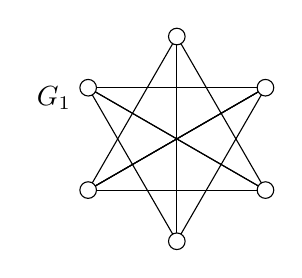
\begin{tikzpicture}[scale=1.3]
\foreach \i in {0,1,2,...,6}{
	\draw  (\i*60+30:1)-- (\i*60+150:1);
	\draw  (\i*60+30:1)-- (\i*60+210:1);
}
\foreach \i in {0,1,2,...,5}{\vertex[fill=white] (\i) at (\i*60+30:1){};

}
\node at (-1.2,.4){$G_1$};
\end{tikzpicture}

\textbf{Proof:} Consider graph $H$, which illustrates a proper coloring on 3 colors.

\begin{align*}
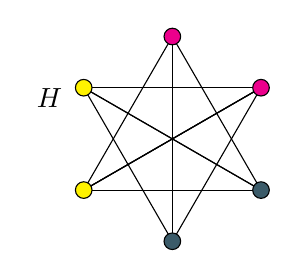
\begin{tikzpicture}[scale=1.3]
\foreach \i in {0,1,2,...,6}{
	\draw  (\i*60+30:1)-- (\i*60+150:1);
	\draw  (\i*60+30:1)-- (\i*60+210:1);
}
\vertex [fill=magenta] at (30:1)  {};
\vertex [fill=magenta] at (90:1)  {};
\vertex [fill= yellow] at (150:1)  {};
\vertex [fill=yellow] at (210:1)  {};
\vertex [fill={rgb:red,53;green,81;blue,94}] at (270:1)  {};
\vertex [fill={rgb:red,53;green,81;blue,94}] at (330:1)  {};
\node at (-1.2,.4){$H$};
\end{tikzpicture}
\end{align*}

If we try to make a proper coloring of the graph $G_1$ on $2$ colors we have a problem because of the odd cycles in $A$ below,
\begin{align*}
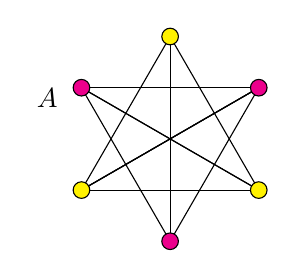
\begin{tikzpicture}[scale=1.3]
\foreach \i in {0,1,2,...,6}{
	\draw  (\i*60+30:1)-- (\i*60+150:1);
	\draw  (\i*60+30:1)-- (\i*60+210:1);
}
\vertex [fill=magenta] at (30:1)  {};
\vertex [fill=yellow] at (90:1)  {};
\vertex [fill= magenta] at (150:1)  {};
\vertex [fill=yellow] at (210:1)  {};
\vertex [fill=magenta] at (270:1)  {};
\vertex [fill=yellow] at (330:1)  {};
\node at (-1.2,.4){$A$};
\end{tikzpicture}
\end{align*}
Thus $\chi(G_1) = 3$.




\vspace{1in}


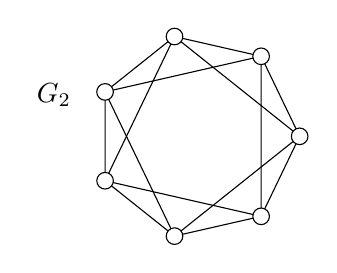
\begin{tikzpicture}[scale=1.3]
\foreach \i in {0,1,2,...,6}{
	\draw  (\i*51.43:1)-- (\i*51.43+51.43:1);
	\draw  (\i*51.43:1)-- (\i*51.43+102.86:1);
}
\foreach \i in {0,1,2,...,6}{\vertex[fill=white] (\i) at (\i*51.43:1){};
}
\node at (-1.4,.4){$G_2$};
\end{tikzpicture}

\textbf{Proof:} Consider graph J, that illustrates a proper coloring of $G_2$ on $4$ colors. 

\begin{align*}
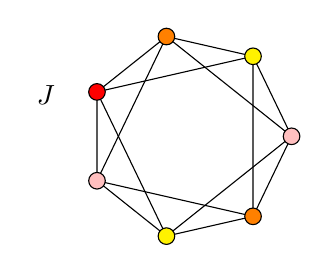
\begin{tikzpicture}[scale=1.3]
\foreach \i in {0,1,2,...,6}{
	\draw  (\i*51.43:1)-- (\i*51.43+51.43:1);
	\draw  (\i*51.43:1)-- (\i*51.43+102.86:1);
}
\vertex [fill=pink] at (0*51.43:1)  {};
\vertex  [fill=yellow] at (1*51.43:1)  {};
\vertex  [fill= orange] at (2*51.43:1)  {};
\vertex [fill=red] at (3*51.43:1)  {};
\vertex  [fill=pink] at (4*51.43:1)  {};
\vertex [fill=yellow] at (5*51.43:1)  {};
\vertex [fill=orange] at (6*51.43:1)  {};
\node at (-1.4,.4){$J$};
\end{tikzpicture}
\end{align*}
Now consider the subgraph $I$,

\begin{align*}
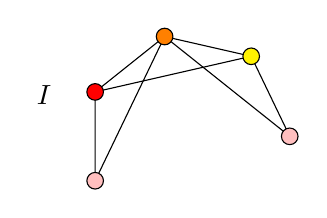
\begin{tikzpicture}[scale=1.3]
\foreach \i in {0,1,2}{
	\draw  (\i*51.43:1)-- (\i*51.43+51.43:1);
	\draw  (\i*51.43:1)-- (\i*51.43+102.86:1);
}
	\draw  (3*51.43:1)-- (3*51.43+51.43:1);
\vertex [fill=pink] at (0*51.43:1)  {};
\vertex  [fill=yellow] at (1*51.43:1)  {};
\vertex  [fill= orange] at (2*51.43:1)  {};
\vertex [fill=red] at (3*51.43:1)  {};
\vertex  [fill=pink] at (4*51.43:1)  {};
\node at (-1.4,.4){$I$};
\end{tikzpicture}
\end{align*}
There exists no proper coloring of subgraph $I$ with 3 colors, because of the three $C_3$ contained within. Thus $\chi(G_2) = 4$.



\vspace{1in}


\item (Problem 6.3.11) Find $p(K_n-e,k)$ where $e$ is any edge of $K_n.$\\

\textbf{Proof:} The chromatic polynomial for any $K_n$ is denoted by,
\begin{equation*}
p(K_n, k) = x(x-1)(x-2)...(x-n-1)
\end{equation*}
This from the fact that since a completed graph has every vertex adjacent to the others we have to let $\chi(K_n) = n$, and the way to do that is to make sure that $p(K_n, 0\leq k \leq n-1) = 0$. From here all we have to do is use Theorem 6.3.3,
\begin{equation*}
p(G,k) + P(G\cdot e, k) = p(G-e,k)
\end{equation*}
And we get,
\begin{equation*}
 p(G-e,k) = x(x-1)(x-2)...(x-n-2) + x(x-1)(x-2)...(x-n-1).
\end{equation*}



\vspace{1in}

\item (Problem 6.3.15) In the chromatic polynomial of a graph $G,$ prove that if $k^m$ is the smallest power of $k$ that has a nonzero coefficient, then $G$ has $m$ components. \\

\textbf{Proof:} (Induction):

Induction HypothesidInduction Hypothesis: If $k^m$ is the smallest power of $k$ that has a nonzero coefficient of the chromatic polynomial of graph $G$, then $G$ has $m$ components.\\

Base Case: Suppose $e(G) = 0$ then a graph with zero edges on $n$ vertices has the chromatic polynomial, $P(G,k) = k^n$. Since $k^n$ is the smallest (only) power of $k$ with a non zero coefficient(coefficient is 1), and we know that $G$ has $n$ components, because it has $n$ vertices and no edges, Induction Hypothesis is true, when $e(G) = 0$. We will proceed by induction on the number of edges.\\

Induction Step: Now let $e(G) = i$ such that $i \geq 1$ and that Induction Hypothesis holds for all $G$ where $e(G) = i-1$, such that $i \geq 1$. By Theorem 6.3.3, \begin{equation*}
p(G,k) = p(G-e,k) - P(G\cdot e, k)
\end{equation*}
Since both graphs $G-e$ and $G\cdot e$ have $i-1$ edges we can apply proposition $A$. Here there are 2 cases, Case 1: where $G-e$ results in a disconnected graph. Case 2: Where $G-e$ results in a connected graph.\\

Case 1: $G-e$ is disconnected. If $G-e$ is disconnected we can assume that the chromatic polynomials are of the form,
\begin{equation*}
p(G-e,k) = k^n - (e(g) - 1)k^{n-1}+\sum_{i  = 2}^{n-2}(-1)^{n-1}a_ik^i
\end{equation*}
\begin{equation*}
p(G \cdot e,k) = k^{n-1} - (e(g) - 1)k^{n-2}+\sum_{j  = 1}^{n-3}(-1)^{n-1-j}b_jk^j
\end{equation*}
Expanding, the sums so we can see the last few terms,
\begin{equation*}
p(G-e,k) = k^n - (e(g) - 1)k^{n-1}+...-a_3k^3+a_2k^2
\end{equation*}
\begin{equation*}
p(G \cdot e,k) = k^{n-1} - (e(g) - 1)k^{n-2}+...-b_2k^2+b_1k
\end{equation*}
We can see that the chromatic polynomial for $G-e$ has $k^2$ as the smallest power of $k$ which makes since because Induction Hypothesis holds for graphs $G$ such that $e(G) = i-1$ and since $G$ is a connected graph and $G-e$ is disconnected, $G-e$ must have 2 components.  Applying Theorem 6.3.3 we get, 
\begin{align*}
p(G,k) &= (k^n - (e(g) - 1)k^{n-1}+...-a_3k^3+a_2k^2) - ( k^{n-1} - (e(g) - 1)k^{n-2}+...-b_2k^2+b_1k)\\
&= k^n-(e(g)-1+1)k^{n-1}+(a_{n-2} +(e(g)-1)k^{n-2} - ... -b_1k
\end{align*}Since $b_1$ is non zero we have shown that $G$ is one component, which is true given our claim that $G-e$ is disconnected.
Thus Induction Hypothesis holds in the case that $G-e$ is disconnected. \\\\

Case 2: $G-e$ is a connected graph.  If $G-e$ is connected we can assume that the chromatic polynomials are of the form,
\begin{equation*}
p(G-e,k) = k^n - (e(g) - 1)k^{n-1}+\sum_{i  = 1}^{n-2}(-1)^{n-1}a_ik^i
\end{equation*}
\begin{equation*}
p(G \cdot e,k) = k^{n-1} - (e(g) - 1)k^{n-2}+\sum_{j  = 1}^{n-3}(-1)^{n-1-j}b_jk^j
\end{equation*}
Expanding, the sums so we can see the last few terms,
\begin{equation*}
p(G-e,k) = k^n - (e(g) - 1)k^{n-1}+...-a_3k^3+a_2k^2 - a_1k 
\end{equation*}
\begin{equation*}
p(G \cdot e,k) = k^{n-1} - (e(g) - 1)k^{n-2}+...-b_2k^2+b_1k
\end{equation*}
Applying Theorem 6.3.3 we get, 
\begin{align*}
p(G,k) &= (k^n - (e(g) - 1)k^{n-1}+...-a_3k^3+a_2k^2- a_1k) - ( k^{n-1} - (e(g) - 1)k^{n-2}+...-b_2k^2+b_1k)\\
&= k^n-(e(g)-1+1)k^{n-1}+(a_{n-2} +(e(g)-1)k^{n-2} - ... -(a_1+b_1)k
\end{align*}
Since $a_1+b_1$ is non zero we have shown that $G$ is one component, which is true given our claim that $G-e$ is connected.
Thus Induction Hypothesis holds in the case that $G-e$ is connected. 
\vspace{1in}

\end{enumerate}
\end{document}
